%% In the documentclass line, replace "noanswers" with "answers" to view the key.

\documentclass[noanswers]{exam}
\usepackage[utf8]{inputenc}

\title{Chapter 11 Practice Problems}
\author{Section 11.3}
\date{STAT 2300}

\usepackage[bottom=2.2cm, left=2.2cm, right=2.2cm, top=2.2cm]{geometry}
%\usepackage[paperheight=11in, paperwidth=17in, margin=1in]{geometry}
\usepackage{dsfont}
\usepackage{amsmath}
\usepackage{amssymb}
\usepackage{amsthm}
\usepackage{array}
\usepackage{stmaryrd}
\usepackage{pgfplots}
\pgfplotsset{width=10cm,compat=1.9}
\usepackage{multicol}
\setlength{\columnsep}{1in}
\usepackage{nicefrac}

\usepackage{multirow}
\usepackage{enumitem}[shortlabels]
\usepackage{tabu}
\definecolor{purp}{RGB}{102,0,204}
\usepackage{tabularx}
\newcolumntype{C}{>{\centering\arraybackslash $}X<{$}}
\usepackage{wrapfig}
\usepackage[export]{adjustbox}


\makeatletter
\pagestyle{headandfoot}
\firstpageheader{\@date}{\@title}{\@author}
\firstpageheadrule
\runningfootrule
\runningfooter{}{\thepage\ / \numpages}{\@title}
\makeatother

\newcommand{\abs}[1]{\left|#1\right|}
\newcommand{\mat}[4]{\left( \begin{tabular}{>{$}c<{$} >{$}c<{$}} #1&#2 \\ #3&#4 \end{tabular} \right)}
\newcommand{\msc}[1]{\mathds{#1}}
\newcommand{\Z}{\mathds{Z}}
\newcommand{\R}{\mathds{R}}
\newcommand{\N}{\mathds{N}}
\newcommand{\Q}{\mathds{Q}}
\newcommand{\C}{\mathds{C}}
\newcommand{\so}{\implies}
\newcommand{\set}[2]{\left\{ #1 \:|\: #2 \right\}}
\newcommand{\bso}{\Longleftarrow}
\newcommand{\ra}{\rightarrow}
\newcommand{\gen}[1]{\left\langle #1 \right\rangle}
\newcommand{\olin}[1]{\overline{#1}}
\newcommand{\Img}[1]{\text{Im}\left(#1\right)}
\newcommand{\llra}{\longleftrightarrow}
\newcommand{\lra}{\longrightarrow}
\newcommand{\xra}[1]{\xrightarrow{#1}}
\newcommand{\wo}{\setminus}
\newcommand{\mcal}[1]{\mathcal{#1}}
\newcommand{\Aut}[1]{\text{Aut}\left(#1\right)}
\newcommand{\Inn}[1]{\text{Inn}\left(#1\right)}
\newcommand{\syl}[2]{\text{Syl}_{#1}(#2)}
\newcommand{\norm}[1]{\left\|#1\right\|}
\newcommand{\infnorm}[1]{\left\|#1\right\|_{\infty}}
\newcommand{\xn}{\{x_n\}}
\newcommand{\sig}{\sigma}
\newcommand{\id}{\text{id}}
\newcommand{\ep}{\epsilon}
\newcommand{\st}{\text{ s.t. }}
\newcommand{\ran}[1]{\text{Ran}(#1)}
\newcommand{\nCr}[2]{\binom{#1}{#2}}
\newcommand{\Exr}[1]{\paragraph{Exercise #1:}}
\newcommand{\pg}{\paragraph{}}
\newcommand{\ulin}[1]{\underline{#1}}
\newcommand{\tc}[1]{\textcolor{purp}{#1}}

% Solution Specs
\unframedsolutions
\renewcommand{\solutiontitle}{}
\SolutionEmphasis{\color{purp}}
\CorrectChoiceEmphasis{\color{purp}\bfseries}
\setlength\fillinlinelength{0in}

%\begin{solution}[\stretch{1}]
%	hurp durp flurp
%\end{solution}

%\pagestyle{empty}

\renewcommand{\arraystretch}{2}
\usepackage{cancel}

\usepackage{scalerel}

\begin{document}

\noindent\begin{tabular}{@{}p{.3in}p{3in}@{}}
Name: & \hrulefill
\end{tabular}

\vspace{2mm}

\begin{questions} 

\question The head of a Biology Department at a large university wants to know how non-transfer students and transfer students differ in terms of their performance on a test that all incoming biology majors have to take. She collected the following data from a random sample of students in the department and summarized their test scores. There are roughly 2500 non-transfer students and 1500 transfer students in the Biology Department.

\begin{center}
\begin{tabular}{c|c|c|c}
 & \textbf{Mean} & \textbf{SD} & \textbf{Sample Size}\\
\hline
Non-Transfer Students & 41.48 & 6.03 & 119 \\
\hline
Transfer Students & 40.79 & 6.79 & 69
\end{tabular}
\end{center}

\begin{parts}

\part What are we estimating? (Define the parameters of interest.)

\begin{solution}[\stretch{1}]

\vspace{1mm}

We are estimating $\mu_{\scaleto{N}{3pt}}-\mu_{\scaleto{T}{3pt}}$, where 

$\mu_{\scaleto{N}{3pt}}=$ the true mean test score on the biology test for non-transfer students and

$\mu_{\scaleto{T}{3pt}}=$ the true mean test score on the biology test for transfer students.

\vspace{3mm}

\end{solution}

\part Verify that the necessary conditions for inference have been met.

\begin{solution}[\stretch{1}]

\vspace{1mm}

\begin{enumerate}
	\item Independent samples --- stated that students were randomly sampled from the biology department.
	
	\item $n_{\scaleto{N}{3pt}}=119< 0.05(2500)=125$ ($<5$\% of non-transfer students) and
	
	$n_{\scaleto{T}{3pt}}=69<0.05(1500)=75$ ($<5$\% of transfer students). 
	
	\item $n_{\scaleto{N}{3pt}}=125>30$ and $n_{\scaleto{T}{3pt}}=69 > 30$ 
\end{enumerate}

\vspace{3mm}

\end{solution}

\part Find a point estimate for the difference in mean biology test score.

\begin{solution}[\stretch{1}]

\vspace{3mm}

$\overline{x}_{\scaleto{N}{3pt}}-\overline{x}_{\scaleto{T}{3pt}}=41.48-40.79=0.69$

\vspace{3mm}

\end{solution}

\part Find the standard error for this difference.

\begin{solution}[\stretch{1}]

\vspace{1mm}

${\scaleto{\sigma}{6pt}}_{\overline{x}_{\scaleto{N}{3pt}}-\overline{x}_{\scaleto{T}{3pt}}}=\displaystyle\sqrt{\frac{s_{\scaleto{N}{3pt}}^2}{n_{\scaleto{N}{3pt}}}+\frac{s_{\scaleto{T}{3pt}}^2}{n_{\scaleto{T}{3pt}}}}=\sqrt{\frac{6.03^2}{119}+\frac{6.79^2}{69}}=0.98678$

\vspace{1mm}

\end{solution}

\part Suppose that JMP software calculates a 95\% confidence interval for $\mu_{\scaleto{T}{4pt}}-\mu_{\scaleto{N}{4pt}}$ to be $(-2.069, 0.689)$. What is the confidence interval for $\mu_{\scaleto{N}{4pt}}-\mu_{\scaleto{T}{4pt}}$?

\begin{solution}[\stretch{1}]

\vspace{3mm}

$(-0.689, 2.069)$

\vspace{3mm}

\end{solution}

\part Interpret your confidence interval in Part (e). 

\begin{solution}[\stretch{1}]

\vspace{3mm}

We are 95\% confident that the true mean biology test score for non-transfer students is between $0.689$ points lower and $2.069$ points higher than the true mean biology test score for transfer students. (i.e.\ that the true difference in sample means is between $-0.689$ and 2.069.)

\vspace{3mm}

\end{solution}

\part Can we conclude that non-transfer students do better on average than transfer students?

\begin{solution}[\stretch{1}]

\vspace{3mm}

No, we cannot conclude that $\mu_{\scaleto{N}{3pt}}>\mu_{\scaleto{T}{3pt}}$ because zero is contained in the interval. 

\vspace{3mm}

\end{solution}

\end{parts}

\newpage

\question Do people walk at different speeds in the airport depending on whether they are departing (getting on a plane) or arriving (getting off a plane)? Researcher Seth B.\ Young measured the walking speeds of different travelers in San Francisco International Airport and Cleveland Hopkins International Airport. His findings are summarized in the following table.

\begin{center}
\begin{tabular}{c|c|c|c}
 & \textbf{Mean (ft/min)} & \textbf{SD (ft/min)} & \textbf{Sample Size}\\
\hline
Departure & 259.2 & 60.3 & 35 \\
\hline
Arrival & 268.9 & 39.9 & 35
\end{tabular}
\end{center}

\begin{parts}
\part Definte the parameters of interest and state the null and alternative hypothesis.

\begin{solution}[\stretch{1}]

\vspace{3mm}

$\mu_{\scaleto{D}{3pt}}=$ true mean walking speed of departing airport travelers

$\mu_{\scaleto{A}{3pt}}=$ true mean walking speed of arriving airport travelers

\vspace{3mm}

$H_0: \mu_{\scaleto{D}{3pt}}=\mu_{\scaleto{A}{3pt}}$ versus $H_a: \mu_{\scaleto{D}{3pt}}\neq\mu_{\scaleto{A}{3pt}}$

\vspace{3mm}

\end{solution}

\part Is the normality condition for inference met?

\begin{solution}[\stretch{1}]

\vspace{3mm}

Yes, because $n_{\scaleto{D}{3pt}}=35>30$ and $n_{\scaleto{A}{3pt}}=35>30$.

(This could also be satisfied if you were provided with roughly linear normal quantile plots.)

\vspace{3mm}

\end{solution}

\part Calculate the test statistic that could be used to compare these two means in a hypothesis test.

\begin{solution}[\stretch{1}]

\vspace{3mm}

$t_0=\displaystyle \frac{\overline{x}_{\scaleto{D}{3pt}}-\overline{x}_{\scaleto{A}{3pt}}}{\sqrt{\frac{s_{\scaleto{D}{3pt}}^2}{n_{\scaleto{D}{3pt}}}+\frac{s_{\scaleto{A}{3pt}}^2}{n_{\scaleto{A}{3pt}}}}}=\frac{259.2-268.9}{\sqrt{\frac{60.3^2}{35}+\frac{39.9^2}{35}}}=-0.794$

\vspace{3mm}

\end{solution}




\part You generate the following JMP output to test the hypotheses defined in Part (a). 

\begin{center}
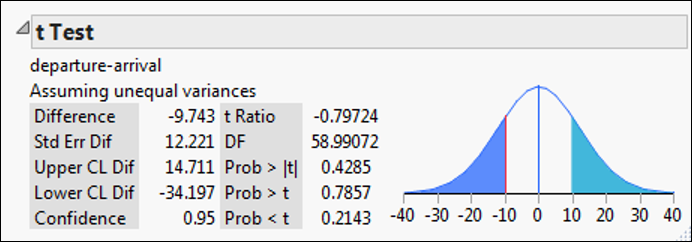
\includegraphics[scale=.55]{STAT_2300_Practice_11-3_JMP.PNG}
\end{center}

What is the p-value for the test?

\begin{solution}[\stretch{1}]

\vspace{3mm}

p-value $=0.4285$ (Select the two-tailed test option.)

\vspace{3mm}

\end{solution}

\part State your conclusion regarding the hypothesis test in context of the problem.

\begin{solution}[\stretch{1}]

\vspace{3mm}

We do not reject $H_0$ because the p-value $>0.05$ ($1-0.95$). At the 5\% significance level, there is insufficient evidence to conclude that people walk at different speeds (on average) whether they are departing or arriving.

\vspace{3mm}

\end{solution}

\part If a 95\% confidence interval for the difference is found, would it contain zero? Explain.

\begin{solution}[\stretch{1}]

\vspace{3mm}

Yes, because there is not a statistically significant difference in the mean walking speeds at the 5\% level.

\vspace{3mm}

\end{solution}

\end{parts}

\end{questions}
%-----------------------------------------------------------------------------%

\end{document}
